
% ----------------------------------------------------------------------
%  Pracovní úkoly
% ----------------------------------------------------------------------
\section{Pracovní úkoly}

\begin{enumerate}
\item S využitím krystalu LiF jako analyzátoru proveďte měření následujících rentgenových spekter:

\begin{enumerate}
    \item Rentgenka s Cu anodou.

    \begin{enumerate}
        \item proměřte krátkovlnné oblasti spekter brzdného záření při napětích 15 kV/1 mA, 25 kV/0,8 mA, 30 kV/0,8 mA, 33 kV/0,8 mA. K měření používejte tyto parametry: clonu o průměru 2 mm, interval Braggova úhlu pro 15 kV v rozmezí (10° – 15°) s krokem 0.2° a dobou expozice 8 s a pro ostatní napětí interval Braggova úhlu (3° – 10°) s krokem 0,2° a dobou expozice 5 s;

        \item proměřte charakteristická spektra rentgenky při napětích 15 kV/1 mA a 33 kV/0,8 mA. K měření používejte tyto parametry: clonu o průměru 2 mm, interval Braggova úhlu (15° – 30°), krok 0,1° a dobu expozice 2 s;

        \item proměřte tvar spektra s Zr absorbérem. K měření používejte tyto parametry: clonu s Zr absorbérem tloušťky 0,05 mm, interval Braggova úhlu (3° – 30°), krok 0,1° a dobu expozice 2 s;

        \item proměřte tvar spektra s Ni absorbérem. K měření používejte tyto parametry: clonu s Ni absorbérem tloušťky 0,01 mm, interval Braggova úhlu (3° – 30°), krok 0,1° a dobu expozice 2 s.
    \end{enumerate}

\item Rentgenka s Fe anodou

    \begin{enumerate}
        \item proměřte charakteristické spektrum rentgenky při napětí 33 kV/0,8 mA. K měření používejte tyto parametry: clonu o průměru 2 mm, interval Braggova úhlu (3° – 30°), krok 0,1° a dobu expozice 2 s;

        \item proměřte tvar spektra s Zr absorbérem. K měření používejte tyto parametry: clonu s Zr absorbérem tloušťky 0,05 mm, interval Braggova úhlu (3° – 30°), krok 0,1° a dobu expozice 3 s.
    \end{enumerate}

\item Rentgenka s Mo anodou.

    \begin{enumerate}
        \item proměřte charakteristické spektrum rentgenky při napětí 33 kV/0.8 mA. K měření používejte tyto parametry: clonu o průměru 2  mm, interval Braggova úhlu (3° – 35°), krok 0,1° a dobu expozice 3 s.
    \end{enumerate}

\item Rentgenka s Cu anodou:

    \begin{enumerate}
        \item proměřte charakteristické spektrum rentgenky při napětí 33 kV/0,8 mA v intervalu Braggova úhlu (42° – 51°). K měření používejte tyto parametry: clonu o průměru 2 mm, krok 0,1° a dobou expozice 2 s.
    \end{enumerate}
    
\end{enumerate}

\item Interpretujte naměřené výsledky (pro mezirovinnou vzdálenost krystalu LiF používejte hodnotu d = 201,4 pm):

\begin{enumerate}
    \item Krátkovlnná mez brzdného záření

    \begin{enumerate}
        \item Ze změřených mezních vlnových délek (respektive frekvencí) určete hodnotu Planckovy konstanty a oceňte přesnost měření
    \end{enumerate}

\item Moseleyův zákon

    \begin{enumerate}
        \item Přesvědčte se, že naměřené úhlové frekvence spektrálních čar K$\alpha$ a K$\beta$ pro různé prvky splňují Moseleyův zákon. Ze směrnice příslušné závislosti určete hodnotu Rydbergovy úhlové frekvence a využitím této hodnoty určete též průměrnou hodnotu stínící konstanty.

        \item Přesvědčte se, že i naměřené polohy absorpčních hran Zr a Ni splňují Moseleyův zákon.

        \item Všimněte si, že absorpční hrana Ni koinciduje se spektrální čarou K$\beta$ mědi; této skutečnosti se využívá v rentgenové difraktografii pro monochromatizaci charakteristického spektra mědi. Z provedeného měření určete filtrační efekt niklu pro čáru K$\beta$.
    \end{enumerate}

\item Úhlová disperze

    \begin{enumerate}
        \item Ze změřených spekter molybdenu určete velikost úhlové disperze pro různé řády difrakce.
    \end{enumerate}
\end{enumerate}

\end{enumerate}

% ----------------------------------------------------------------------
%  Teoretická část
% ----------------------------------------------------------------------
\section{Teoretická část}

Základem celého experimentu je \textbf{Braggova rovnice}, která popisuje difrakci rentgenového záření na krystalové mřížce. Předpokládá se, že záření se "odráží" od soustavy rovnoběžných rovin v krystalu. K zesílení (difrakčnímu maximu) dojde, pokud je dráhový rozdíl paprsků odražených od sousedních rovin roven celočíselnému násobku vlnové délky. To vyjadřuje vztah (1):
%
$$ 2d \sin \vartheta = n\lambda $$
%
kde $d$ je vzdálenost difrakčních rovin, $\vartheta$ je Braggův úhel (úhel dopadu), $n$ je řád difrakce a $\lambda$ je vlnová délka záření.

Rentgenové záření v rentgence vzniká dvěma hlavními mechanismy:

\begin{enumerate}
    \item \textbf{Brzdné záření}: Vzniká při interakci urychlených elektronů s materiálem anody, kdy elektrony postupně ztrácejí kinetickou energii. Toto záření má spojité spektrum. Spektrum má ostrou \textbf{krátkovlnnou hranici $\lambda_m$}. Ta odpovídá situaci, kdy jediný foton odnese celou kinetickou energii elektronu $E_k = eU_a$. Z této hranice lze určit Planckovu konstantu pomocí vztahu (2):
    %
    $$ \frac{hc}{\lambda_m} = eU_a $$
    %
    \item \textbf{Charakteristické záření}: Při dostatečně vysoké energii urychlených elektronů dochází k vyražení elektronu z vnitřních slupek atomů anody (např. slupky K). Volné místo je následně zaplněno elektronem z vyšší slupky (L, M, \dots), což vede k emisi fotonu s diskrétní energií. Takto vznikají série čar, např. $K_{\alpha}$ (přechod L$\to$K) a $K_{\beta}$ (přechod M$\to$K).
\end{enumerate}

Poloha těchto čar závisí na atomovém čísle $Z$ materiálu anody a řídí se \textbf{Moseleyovým zákonem}. Ten lze podle \cite{bib:studijni-text} pro přechody do slupky K (n=1) ze slupky L (n=2) vyjádřit vztahem (3):
%
$$ \sqrt{\omega} = \frac{\sqrt{3R_{\omega}}}{2}(Z-s) $$
%
kde $R_{\omega}$ je Rydbergova úhlová frekvence a $s$ je stínící konstanta.

Pro analýzu spekter je důležitá \textbf{úhlová disperze} spektrometru. Ta je definována jako $\partial\vartheta / \partial\lambda$ a lze ji odvodit z Braggovy rovnice jako vztah (4):
%
$$ \frac{\partial\vartheta}{\partial\lambda} = \frac{n}{2d \cos \vartheta} $$
%
Při průchodu záření materiálem (absorbérem) dochází k jeho útlumu. Intenzita záření klesá exponenciálně podle vztahu (5): $I = I_0 e^{-\mu l}$, kde $l$ je tloušťka absorbéru a $\mu$ je \textbf{součinitel útlumu}. Tento součinitel $\mu$ sám závisí na vlnové délce, přičemž vykazuje náhlé skoky u tzv. \textbf{absorpčních hran}.


Chyba je spočtena pomocí metody přenosu chyb \cite{bib:metoda-prenosu-chyb} jako (6)

\begin{equation}
    \nonumber
    \sigma = \sqrt{\sum^n_{i=1} \left( \frac{\partial f}{\partial x_i} \right)^2 \sigma^2_{x_i}}
\end{equation}

% ----------------------------------------------------------------------
%  Výsledky a zpracování měření
% ----------------------------------------------------------------------
\section{Výsledky a zpracování měření}

\subsection{Určení Planckovy konstanty}
Naměřili jsme krátkovlnné oblasti spekter pro Cu anodu podle prvního pracovního úkolu. Z těchto závislostí jsme vybrali hodnoty s lineární závislostí nad nulou. Pouze tyto hodnoty jsme proložili lineární regresí a určili bod ve kterém tato přímka protíná 0 na y-ose. Tyto hodnoty jsme opět zobrazili v grafu v závislosti na urychlovacím napětí. Nakonec jsme závislost $\frac{1}{sin(x/2)}(U)$ proložili lineárním fitem se zafixovaným absolutním členem na 0. X odpovídá úhlu detektoru, který dělíme 2 pro přepočet na úhel přicházejícího svazku. Tato závislost je znázorněna na obrázku \ref{fig:Planck}.

\begin{figure}[!h]
    \centering
    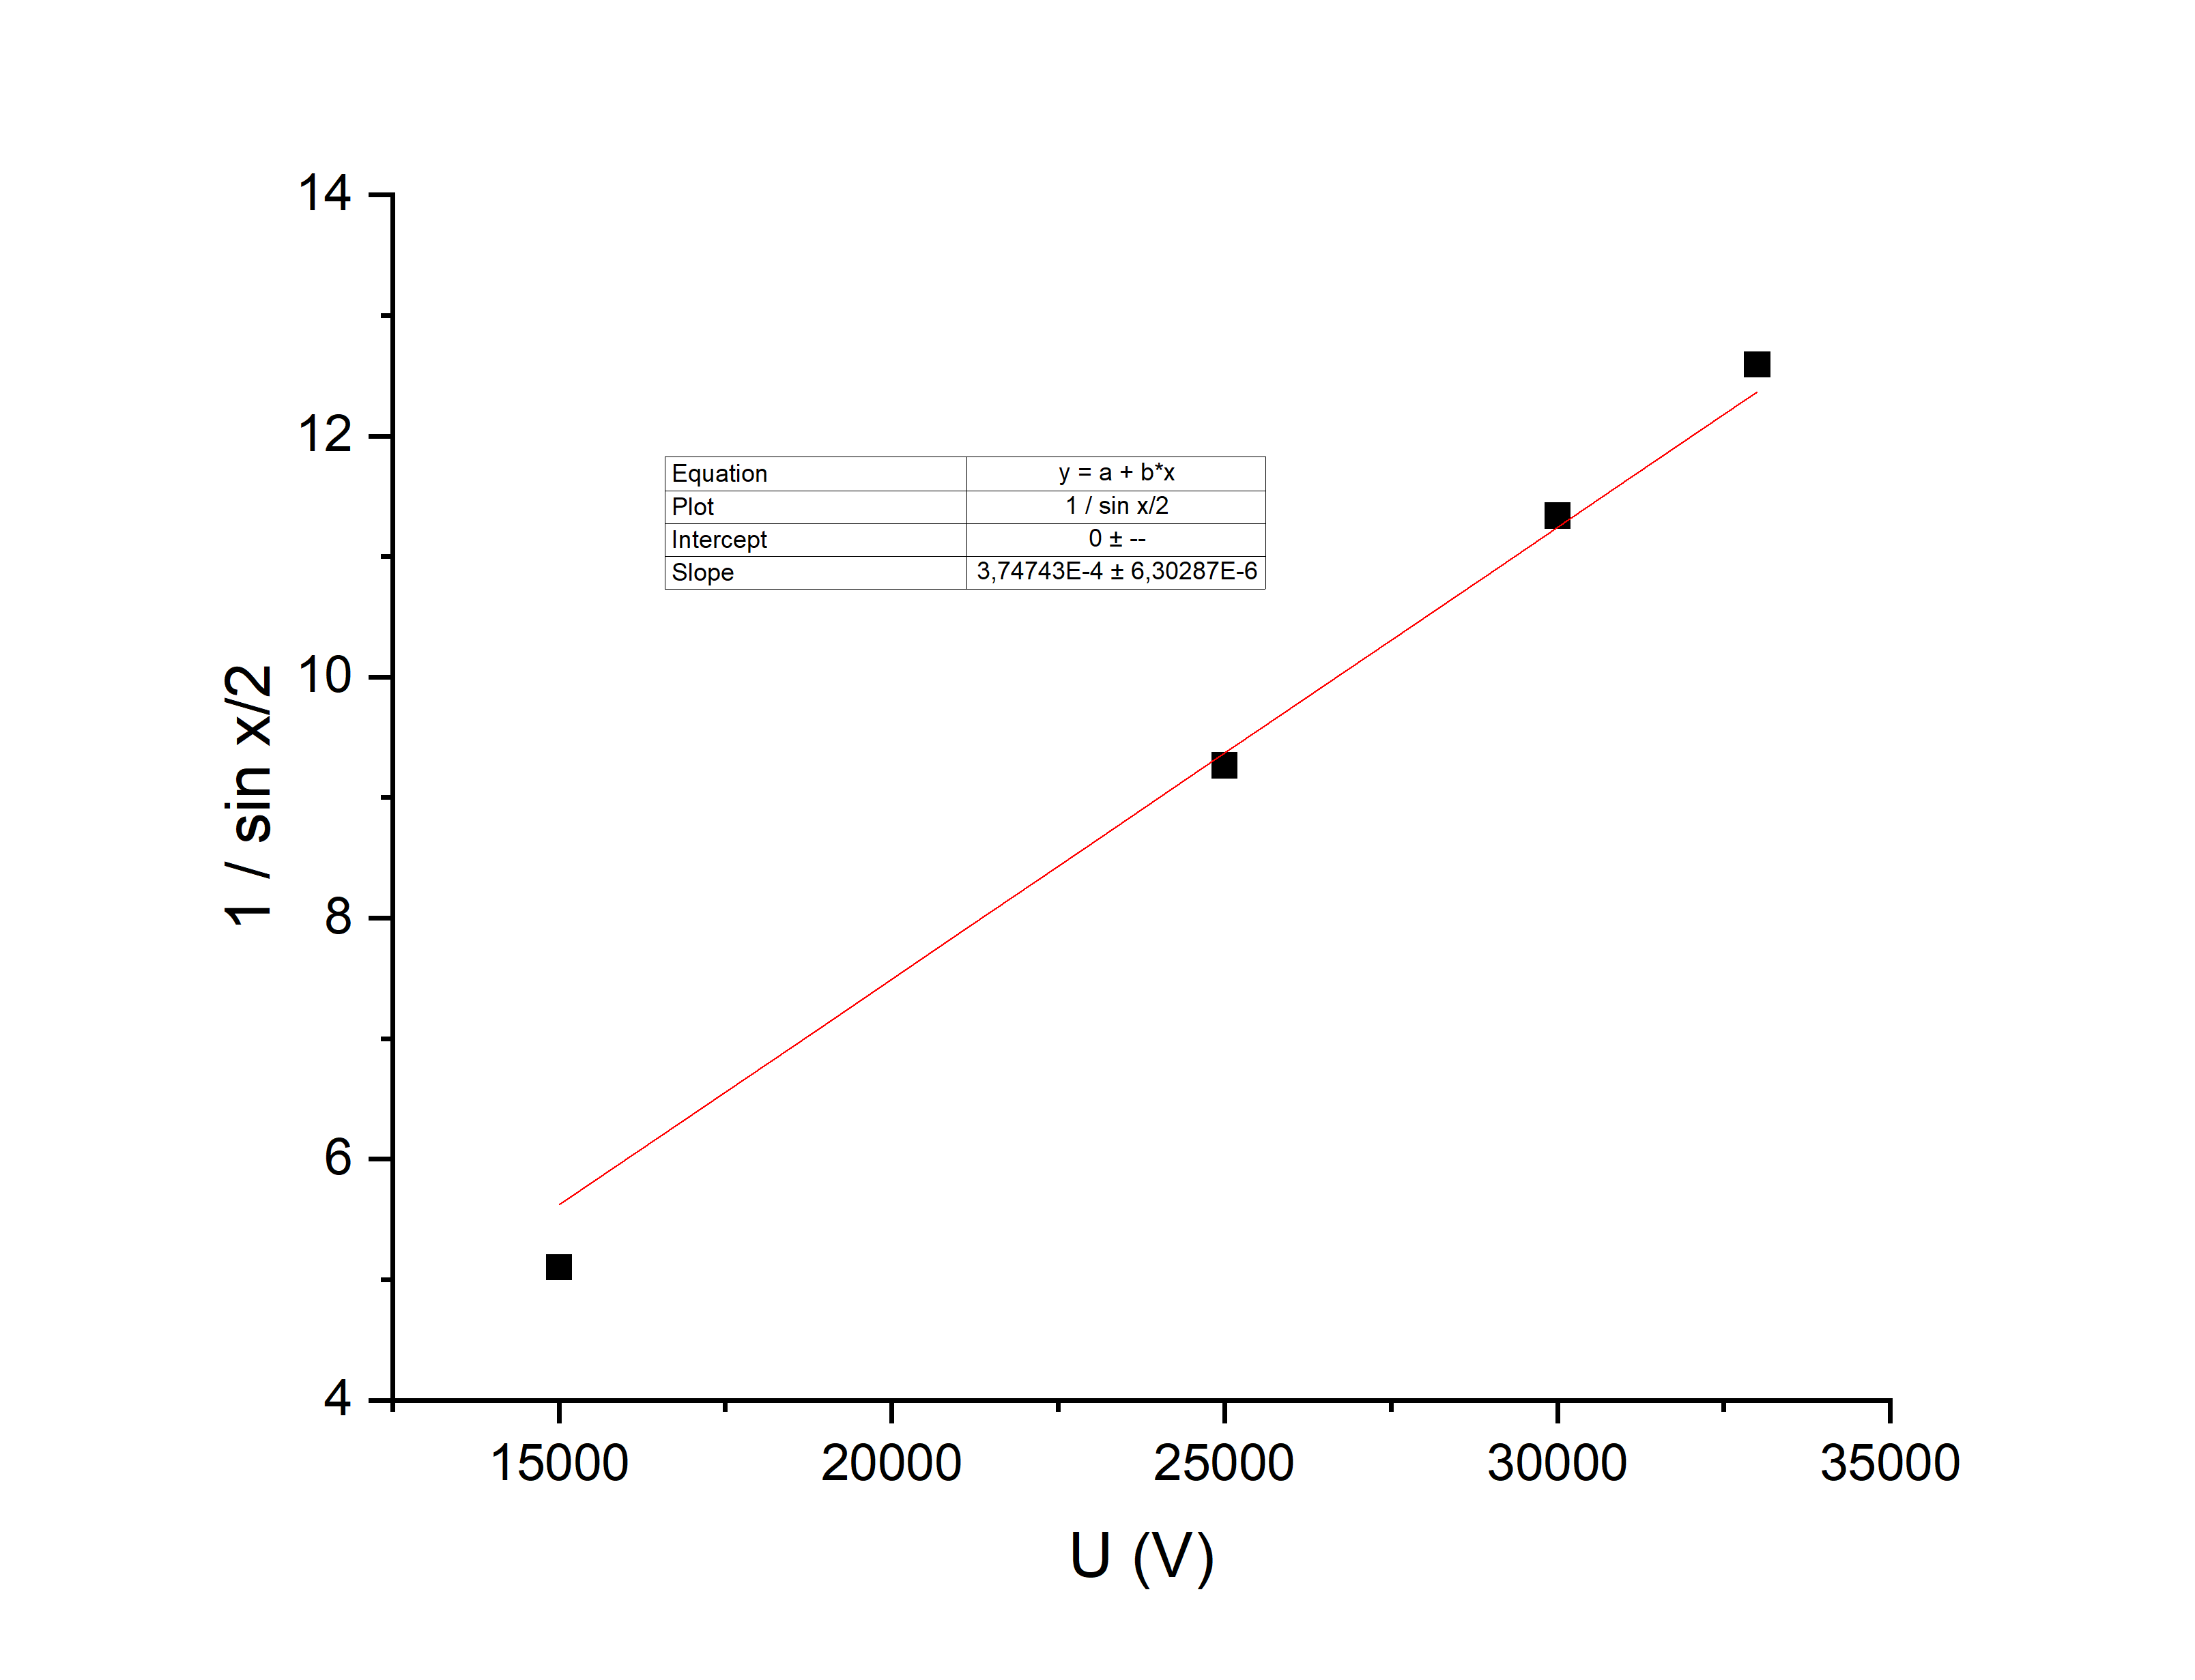
\includegraphics[width=1\linewidth]{A21 - rentgen - kopie/Planck.png}
    \caption{Lineární fit pro určení Planckovy konstanty}
    \label{fig:Planck}
\end{figure}
\newpage
Poté jsme z parametru fitu získali naměřenou hodnotu Planckovy konstanty

\begin{equation}
    \nonumber
    h = (8,1 \pm 0,5) \cdot 10^{-34} \; J \cdot s
\end{equation}


\subsection{Moseleyův zákon}

Proměřili jsme charakteristické spektrum pro anody složené z Fe, Mo a Cu při urychlovacím napětím napětí 33 kV a proudu 0,8 mA. Podle zadání $\cite{bib:zadani}$ jsme pro některá měření použili zr absorbér tloušťky 0,05 mm a Ni absorbér s tloušťkou 0,01 mm. Pokud nebyl použit ani jeden z těchto absorbérů měřili jsme se clonou o průměru 2 mm. Doba expozice pro každý úhel byla nastavena na 2 s pro Fe a Cu, pro Mo 3 s. Naměřené výsledky jsou uvedeny v tabulce \ref{tab:vlnove_delky}. Uvedený úhel je úhel v tabulce je úhel mezi krystalem analyzátoru a přilétávajícím svazkem, který je poloviční oproti úhlu detektoru, který jsme měřili. Pro jednotlivé materiály jsme vypsali také teoretické hodnoty podle tabulek v praktiku.

\begin{table}[h!]
\centering
\caption{Porovnání naměřených a teoretických vlnových délek}
% Specifikace sloupců: l (levý), c (střed), l (levý), r (pravý), r (pravý)
\begin{tabular}{l c l r r}
\hline\hline
% Hlavička tabulky
Použité materiály & Úhel svazku / $^\circ$ & Typ přechodu & $\lambda \pm \Delta\lambda$ / pm & $\lambda_{\text{teor}}$ / pm \\
\hline
% Data - Cu
Cu 15 kV & 19,9 & K$_{\beta}$, n=1 & $137,1 \pm 0,7$ & 140,4 \\
         & 22,2 & K$_{\alpha}$, n=1 & $152,2 \pm 0,7$ & 154,1 \\
\hline
Cu 33 kV & 19,9 & K$_{\beta}$, n=1 & $137,1 \pm 0,7$ & \\
         & 22,1 & K$_{\alpha}$, n=1 & $151,5 \pm 0,7$ & \\
         & 43,3 & K$_{\beta}$, n=2 & $138,1 \pm 0,3$ & 139,6 \\ 
         & 49,55 & K$_{\alpha}$, n=2 & $153,3 \pm 0,2$ & 154,9 \\ 
\hline
Cu 33 kV, Zr & 19,9 & K$_{\beta}$, n=1 & $137,1 \pm 0,7$ & \\
             & 22,2 & K$_{\alpha}$, n=1 & $152,2 \pm 0,7$ & \\
\hline
Cu 33 kV, Ni & 19,9 & K$_{\beta}$, n=1 & $137,1 \pm 0,7$ & \\
             & 22,2 & K$_{\alpha}$, n=1 & $152,2 \pm 0,7$ & \\
\hline % <-- Oddělovač
% Data - Fe
Fe 33 kV & 25,8 & K$_{\beta}$, n=1 & $175,3 \pm 0,6$ & 175,3 \\
         & 28,6 & K$_{\alpha}$, n=1 & $192,8 \pm 0,6$ & 194,7 \\
\hline
Fe 33 kV, Zr & 25,7 & K$_{\beta}$, n=1 & $174,7 \pm 0,6$ & \\
             & 28,6 & K$_{\alpha}$, n=1 & $192,8 \pm 0,6$ & \\
\hline % <-- Oddělovač
% Data - Mo
Mo 33 kV & 8,7 & K$_{\beta}$, n=1 & $60,9 \pm 0,7$ & 64,4 \\
         & 9,8 & K$_{\alpha}$, n=1 & $68,6 \pm 0,7$ & 70,4 \\
         & 17,75 & K$_{\beta}$, n=2 & $61,4 \pm 0,3$ & 63,9 \\ 
         & 20,25 & K$_{\alpha}$, n=2 & $69,7 \pm 0,7$ & 71,2\\ 
\hline % <-- Oddělovač  
% Data - Zr
Zr       & 9,7 &                & $67,9 \pm 0,7$ & \\
\hline % <-- Oddělovač
% Data - Ni
Ni       & 19,9 &                & $137,1 \pm 0,7$ & \\
\hline\hline
\end{tabular}
\label{tab:vlnove_delky}
\end{table}

\newpage

Na obrázku \ref{fig:cu-poro-abs} jsou znázorněna charakteristická spektra Cu se clonou, se Zr a Ni absorbérem pro porovnání. Všechny závislosti jsou měřeny při urychlovacím napětí 33 kV.

\begin{figure}[!h]
    \centering
    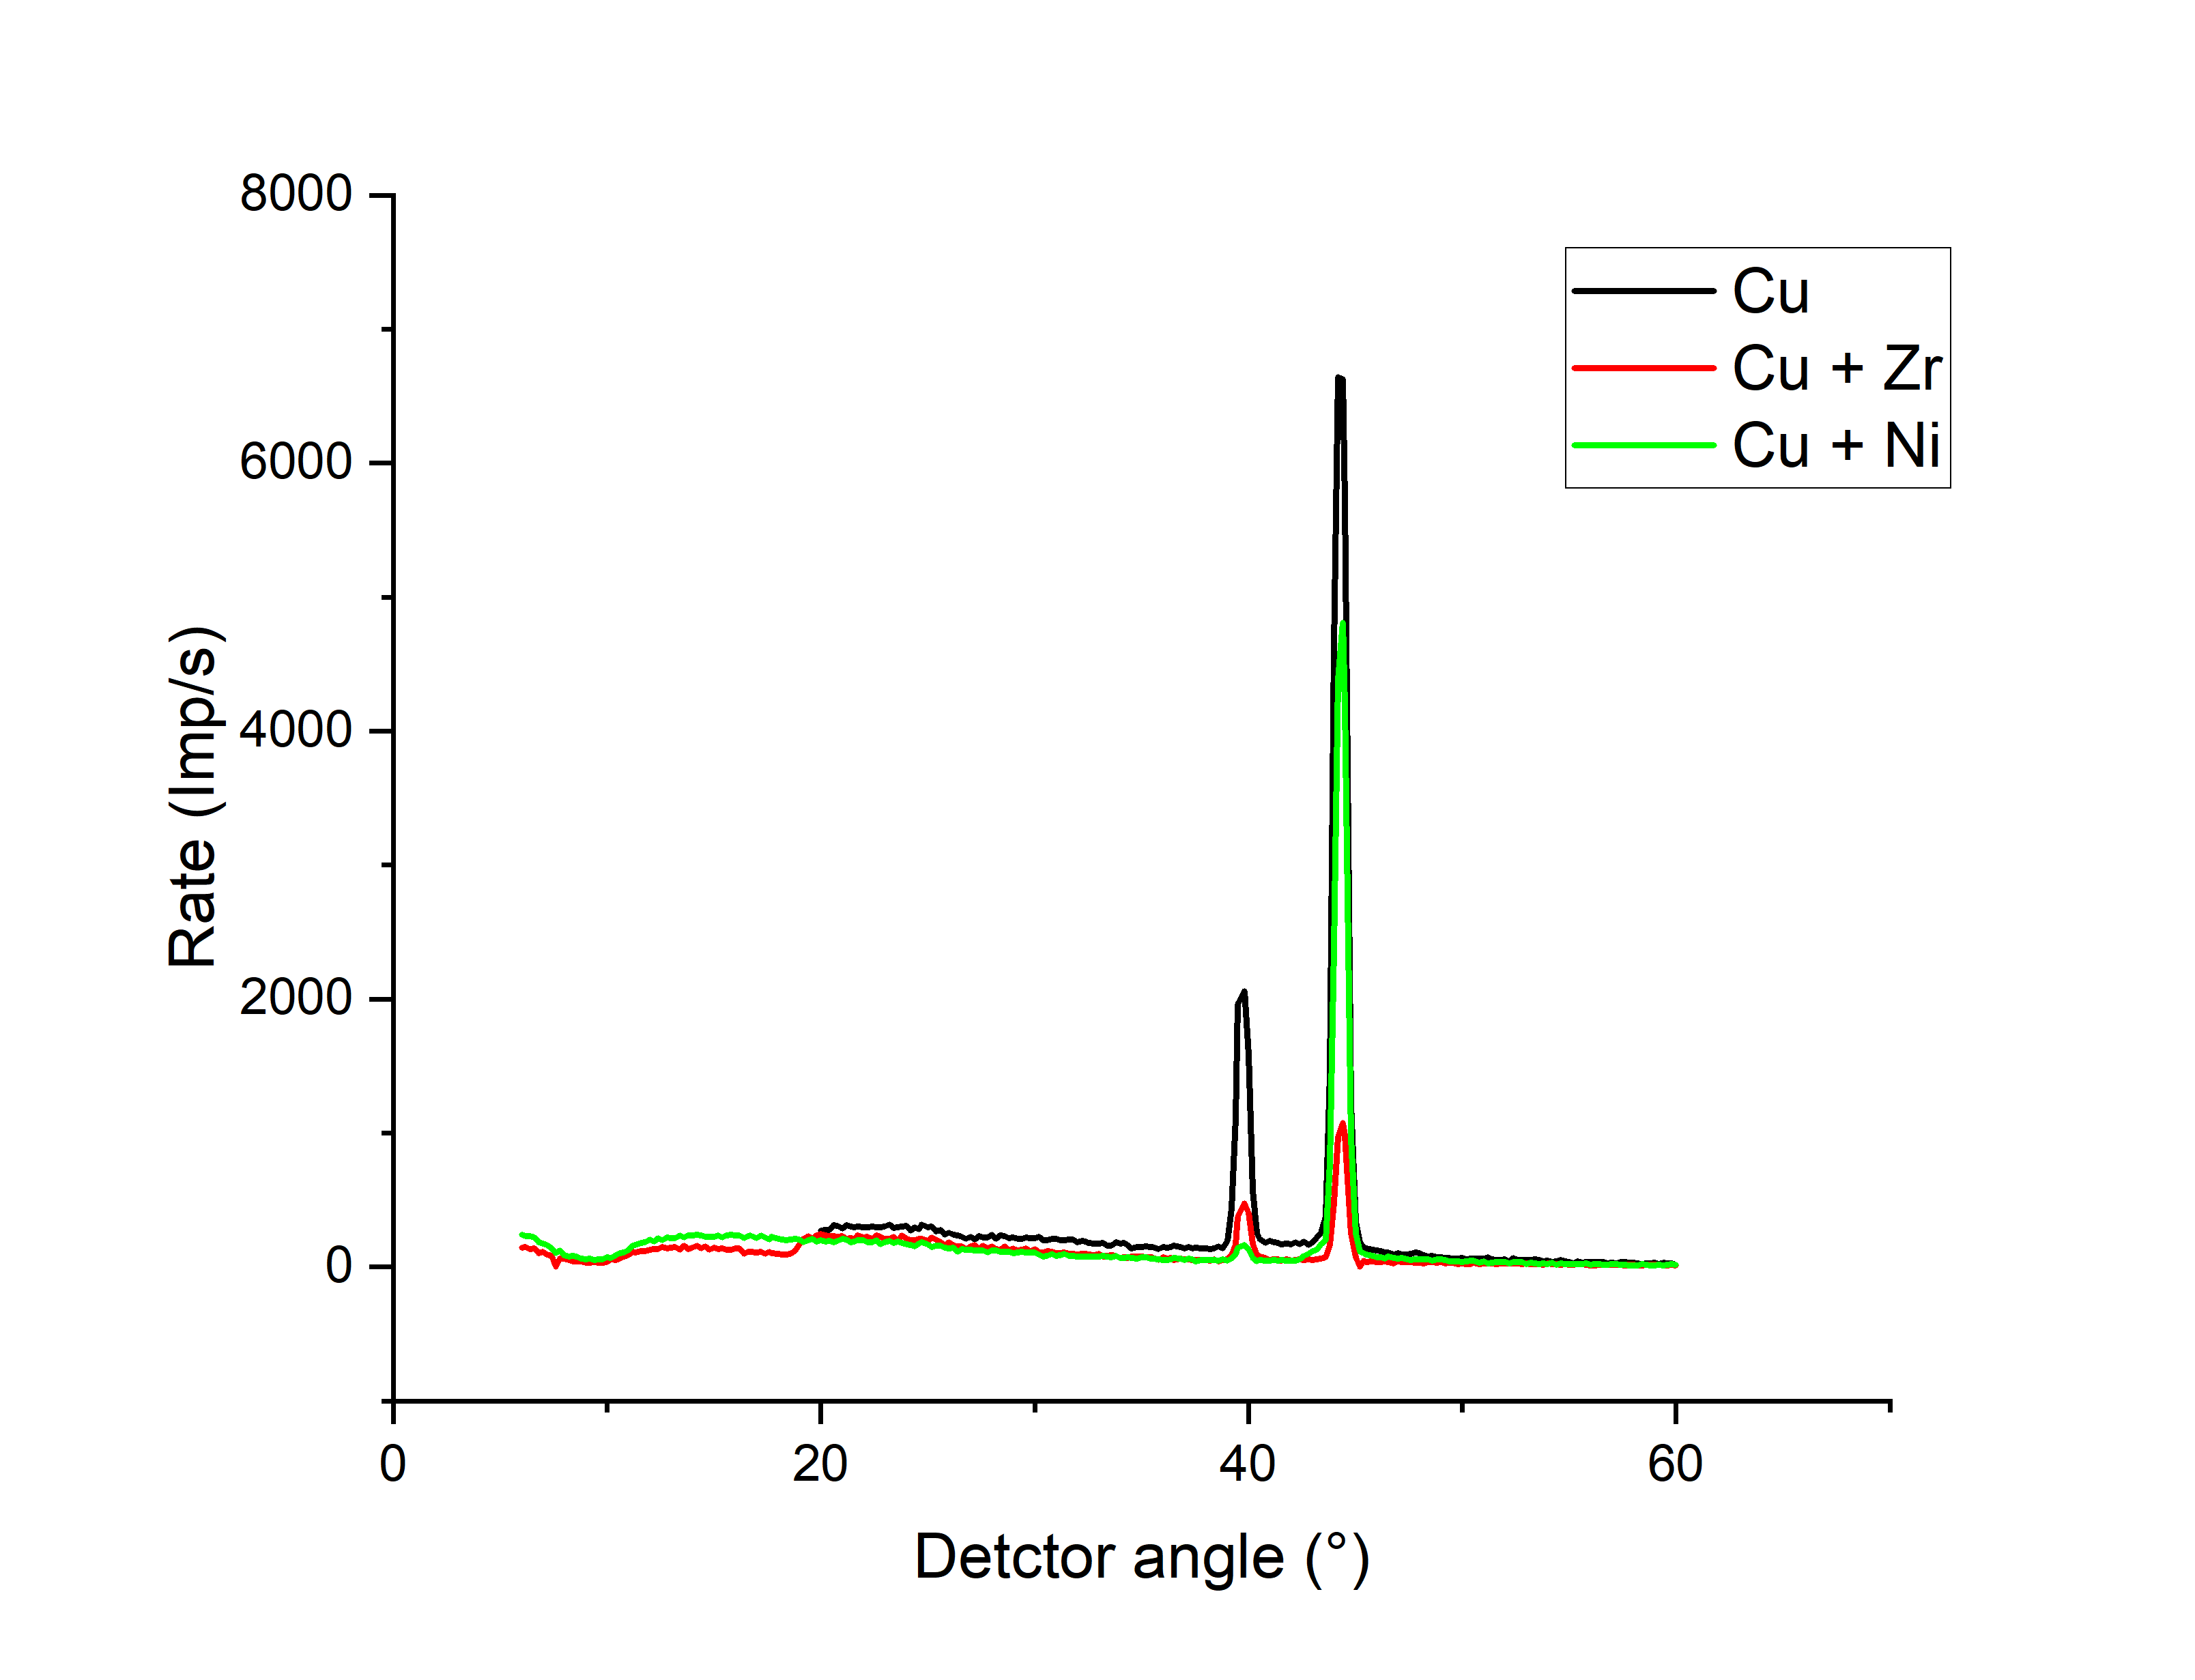
\includegraphics[width=1\linewidth]{A21 - rentgen/Cu provnání s absorbátorama.png}
    \caption{Porovnání charakteristických spekter mědi bez a s absorbéry.}
    \label{fig:cu-poro-abs}
\end{figure}

Vidíme, že naměřené vlnové délky jsou posunuté hodnotou systematicky oproti teoretické hodnotě podle tabulek v praktiku. Zpětně tak můžeme určit systematickou chybu měření. Tato nejistota úhlu přicházejícího svazku pak je 0,5 °. Jak jsme předpokládali krystal LiF není v aparatuře umístěn s naprostou přesností, je ale mírně natočen. Proto jsme při měření pozorovali nenulové hodnoty pro úhly blízké nule, viz. diskuze. Proto v dalších výpočtech již používáme korigované hodnoty. Nejistotu vlnové délky jsme dopočetli podle Gaussově přenosu chyb.

Dále pozorujeme, že Ni filtruje spektrální čáru $K_\beta$. Odečteme, že rate klesl z 2060 Imp/s na 167 Imp/s. Známe tloušťku (0,01 mm) a proto můžeme dopočítat podle (5) $\mu = 251,3 \; mm^{-1}$.

Dále jsme určili Rydbergovu úhlovou frekvenci z naměřených dat a vztahu pro Moseleyův zákon. Z tabulky \ref{tab:vlnove_delky} jsme uvažovali pouze přechody z n=2 do n=1. Na obrázku je znázorněna závislost $\lambda^{-\frac{1}{2}}$ na atomovém čísle $Z$ a proložena lineárním fitem. Závislost tedy odpovídá vztahu $\frac{1}{\sqrt{\lambda}}= a \cdot Z + b$. Výsledky jsou zobrazeny v tabulce \ref{tab:fit_parametry}. Neuvažujeme zde chyby fitu, protože jsme fitovali vždy dvě hodnoty.

\begin{table}[h!]
\centering
\caption{Parametry lineárního fitu Moseleyova zákona}
% Používám zarovnání doprava (r) pro čísla
\begin{tabular}{l r r r r}
\hline\hline
% Hlavička tabulky
Přechod & $A \text{ / } (10^{-3} \text{ pm}^{-1/2})$ & $B \text{ / } (10^{-3} \text{ pm}^{-1/2})$ & $R_{\omega} \text{ / } (10^{16} \text{ s}^{-1})$ & $s$ \\
\hline
% Data
% Předpokládám, že první řádek je K_beta a druhý K_alpha
$K_{\beta}$ & 3,00 & -6,22 & 2,26 & 2,07 \\
$K_{\alpha}$ & 3,27 & -9,79 & 2,69 & 2,99 \\
\hline\hline
\end{tabular}
\label{tab:fit_parametry}
\end{table}

\subsection{Úhlová disperze}
U Mo anody jsme pozorovali 2 řády difrakce. V tabulce jsou zobrazeny naměřené hodnoty. $\theta_1$ značí polohu peaku, při kterém jsme pozorovali přechod $\alpha$, $\theta_2$ pak přechod $\beta$. Uvažujeme již korigované hodnoty o systematickou chybu.

\begin{table}[h!]
\centering
\caption{Shrnutí výsledků s dopočtenými chybami (přepočtené hodnoty $\lambda$)}
% Používám zarovnání doprava (r) pro čísla a (c) pro první sloupec
\begin{tabular}{c r r r r r}
\hline\hline
% Hlavička tabulky
řád ($n$) & $\theta_1 \text{ / } (^\circ)$ & $\theta_2 \text{ / } (^\circ)$ & $\lambda_1 \text{ / } (\text{pm})$ & $\lambda_2 \text{ / } (\text{pm})$ & $\frac{d\theta}{d\lambda} \text{ / } (\text{nm}^{-1})$ \\
\hline
% Data
1 & $10,3 \pm 0,1$ & $9,2 \pm 0,1$ & $72,0 \pm 0,7$ & $64,4 \pm 0,7$ & $2,520 \pm 0,001$ \\
2 & $25,25 \pm 0,1$ & $22,75 \pm 0,1$ & $85,9 \pm 0,7$ & $77,9 \pm 0,7$ & $5,435 \pm 0,003$ \\
\hline\hline
\end{tabular}
\label{tab:vysledky_disperze}
\end{table}

To jsme nakonec porovnali s teoretickými hodnotami:

Pro n=1:
\begin{equation}
    \nonumber
    K_\alpha = 2,525 \; mm^{-1}
\end{equation}

\begin{equation}
    \nonumber
    K_\beta = 2,516 \; mm^{-1}
\end{equation}

Pro n=2:

\begin{equation}
    \nonumber
    K_\alpha = 5,309 \; mm^{-1}
\end{equation}

\begin{equation}
    \nonumber
    K_\beta = 5,234 \; mm^{-1}
\end{equation}

    
% ----------------------------------------------------------------------
%  Diskuse výsledků
% ----------------------------------------------------------------------
\newpage
\section{Diskuse výsledků}
Nenulové hodnoty u nuly - naklonění LiF a průměr detektoru.
Při zpracování dat byla nejprve určena systematická chyba měření úhlu na $+0,5^{\circ}$, která byla přičtena ke všem naměřeným hodnotám. Tato chyba je pravděpodobně způsobena pootočením LiF krystalu.

Určení Planckovy konstanty (kap. 3.1) vedlo k hodnotě $h = (8,1 \pm 0,5) \cdot 10^{-34}\text{ J}\cdot\text{s}$. Tato hodnota neodpovídá tabulkové ani v rámci své chyby. To je zřejmě způsobeno diskutovanou systematickou chybou, která zde nebyla při výpočtu korigována. To je možné doporučit jako případné vylepšení experimentu.

Z Moseleyova zákona (Tab. 2 6) byla určena Rydbergova úhlová frekvence $R_{\omega}(K_{\alpha}) = 2,69 \times 10^{16} \text{ s}^{-1}$ a stínící konstanta $s(K_{\alpha}) = 2,99$7. Tyto hodnoty jsou v rozumném souladu s teorií. Fit závislosti pro ověření tohoto zákona však není dostateční statistický vzorek. Uvažujeme pouze dvě hodnoty. Bylo by možné uvážit i třetí hodnotu pro každý fit pro nízké Z, avšak i v tomto případě nelze hovořit o dostatečném statistickém zpracování. Dostali bychom podobnou situaci.

Měření s Ni absorbérem (Obr. 2 8) potvrdilo jeho filtrační efekt pro čáru $K_{\beta}$ mědi. Pokles intenzity z 2060 Imp/s na 167 Imp/s odpovídá absorpčnímu koeficientu $\mu = 251,3 \text{ mm}^{-1}$, což je v dobré shodě s referenčními hodnotami. Pro Cu anodu s Ni absorbérem jsme tak dosáhli téměř monochromatického záření, kterého se takto využívá v různých aplikacích v praxi.

Pro úhlovou disperzi (Tab. 3) byla pro řád $n=1$ naměřena hodnota $D = 2,520 \text{ nm}^{-1}$, která se shoduje s teoretickým průměrem ($\approx 2,52 \text{ nm}^{-1}$). U řádu $n=2$ je však naměřená hodnota $D = 5,435 \text{ nm}^{-1}$ v nízkém sporu s teorií ($\approx 5,27 \text{ nm}^{-1}$).

Při Mo anodě jsme na grafu objevili pouze 2 difrakční řády s přesvědčivou přesností, avšak lze očekávat že by se pro vyšší měřené úhly mohl vyskytovat i třetí řád.
% ----------------------------------------------------------------------
%  Závěr
% ----------------------------------------------------------------------
\section{Závěr}

V rámci této úlohy byla úspěšně proměřena rentgenová spektra. Z krátkovlnné hrany brzdného záření byla určena Planckova konstanta $h = (8,1 \pm 0,5) \cdot 10^{-34} \text{ J}\cdot\text{s}$.

Z charakteristických spekter byl ověřen Moseleyův zákon. Z fitu dat byly pro přechod $K_{\alpha}$ určeny Rydbergova úhlová frekvence $R_{\omega} = 2,69 \cdot 10^{16} \text{ s}^{-1}$ a stínící konstanta $s = 2,99$.

Měřením s Ni absorbérem byl potvrzen jeho filtrační efekt pro čáru $K_{\beta}$ mědi a byl vypočten lineární absorpční koeficient $\mu = 251,3 \text{ mm}^{-1}$.

Nakonec byla ze spekter molybdenu určena úhlová disperze pro řád $n=1$ jako $D = 2,520 \text{ nm}^{-1}$ a pro řád $n=2$ jako $D = 5,435 \text{ nm}^{-1}$.